\documentclass[t,xcolor=pdftex,dvipsnames,table]{beamer}
\usepackage[]{graphicx}\usepackage[]{color}
%% maxwidth is the original width if it is less than linewidth
%% otherwise use linewidth (to make sure the graphics do not exceed the margin)
\makeatletter
\def\maxwidth{ %
  \ifdim\Gin@nat@width>\linewidth
    \linewidth
  \else
    \Gin@nat@width
  \fi
}
\makeatother

\definecolor{fgcolor}{rgb}{0.345, 0.345, 0.345}
\newcommand{\hlnum}[1]{\textcolor[rgb]{0.686,0.059,0.569}{#1}}%
\newcommand{\hlstr}[1]{\textcolor[rgb]{0.192,0.494,0.8}{#1}}%
\newcommand{\hlcom}[1]{\textcolor[rgb]{0.678,0.584,0.686}{\textit{#1}}}%
\newcommand{\hlopt}[1]{\textcolor[rgb]{0,0,0}{#1}}%
\newcommand{\hlstd}[1]{\textcolor[rgb]{0.345,0.345,0.345}{#1}}%
\newcommand{\hlkwa}[1]{\textcolor[rgb]{0.161,0.373,0.58}{\textbf{#1}}}%
\newcommand{\hlkwb}[1]{\textcolor[rgb]{0.69,0.353,0.396}{#1}}%
\newcommand{\hlkwc}[1]{\textcolor[rgb]{0.333,0.667,0.333}{#1}}%
\newcommand{\hlkwd}[1]{\textcolor[rgb]{0.737,0.353,0.396}{\textbf{#1}}}%
\let\hlipl\hlkwb

\usepackage{framed}
\makeatletter
\newenvironment{kframe}{%
 \def\at@end@of@kframe{}%
 \ifinner\ifhmode%
  \def\at@end@of@kframe{\end{minipage}}%
  \begin{minipage}{\columnwidth}%
 \fi\fi%
 \def\FrameCommand##1{\hskip\@totalleftmargin \hskip-\fboxsep
 \colorbox{shadecolor}{##1}\hskip-\fboxsep
     % There is no \\@totalrightmargin, so:
     \hskip-\linewidth \hskip-\@totalleftmargin \hskip\columnwidth}%
 \MakeFramed {\advance\hsize-\width
   \@totalleftmargin\z@ \linewidth\hsize
   \@setminipage}}%
 {\par\unskip\endMakeFramed%
 \at@end@of@kframe}
\makeatother

\definecolor{shadecolor}{rgb}{.97, .97, .97}
\definecolor{messagecolor}{rgb}{0, 0, 0}
\definecolor{warningcolor}{rgb}{1, 0, 1}
\definecolor{errorcolor}{rgb}{1, 0, 0}
\newenvironment{knitrout}{}{} % an empty environment to be redefined in TeX

\usepackage{alltt}
\newcommand{\SweaveOpts}[1]{}  % do not interfere with LaTeX
\newcommand{\SweaveInput}[1]{} % because they are not real TeX commands
\newcommand{\Sexpr}[1]{}       % will only be parsed by R


%\documentclass[handout,t,xcolor=pdftex,dvipsnames,table]{beamer}  % For handout
\mode<presentation>{
\useoutertheme[subsection=false]{miniframes}
%\beamertemplatenavigationsymbolsempty
\usecolortheme{custom}
\usefonttheme[onlymath]{serif}
\setbeamercovered{invisible}
%\setbeamertemplate{navigation symbols}{}
%\setbeamertemplate{mini frames}{}  % Old one
% Comment out this line to give the header
% \setbeamertemplate{headline}[default]
\setbeamertemplate{caption}[numbered]
%\setbeamertemplate{itemize items}[circle] 
\setbeamertemplate{frametitle continuation}{\frametitle{\color{white}Title}}  % So no tile on subsequent frames, from [allowframebreaks]

%%% CUSTOMISING NAVIATION %%%%
%This customises the navigation to be thin width and just have section headings (not subsections). 
\setbeamertemplate{headline}{%
\leavevmode%
  \hbox{%
    \begin{beamercolorbox}[wd=\paperwidth,ht=2.5ex,dp=1.125ex]{palette tertiary}%   % Tertiary colour is blue
    \insertsectionnavigationhorizontal{\paperwidth}{}{\hskip0pt plus1filll}
    \end{beamercolorbox}%
}}}

\RequirePackage{marvosym}

%%% INCLUDING SOLUTIONS %%%%
%% You can incorporate both questions and solutions in the 
%% same document.  Solutions can be included between the 
%% commands \begin{soln} and \end{soln}
%% To generate a pdf with only the questions uncomment:
%\excludecomment{soln}
\usepackage{comment}
\specialcomment{soln}{\begingroup \vspace{1mm} \sl}{ \leavevmode \endgroup}

%%%% DETAILS FOR PART 1 TITLE PAGE (OLD) %%%%
%\title{\large Part2 - Probability \& Distribution Theory} 
%\subtitle{} 
%\author{\copyright Dr Di Warren 2016} 
%\date{MATH1005 - Statistics}
% \colorlet{Faculty}{Arts}
%\colorlet{Faculty}{MasterBrandRed} % This is only needed if the notes are used for different faculties.
%\colorlet{FacultyText}{White}
% Defines the color of the text used on the title page and ``blocks''
% White for Business; TitlePageBlack for Arts, Pharmacy and Science
%\definecolor{CoolBlack}{rgb}{0.0, 0.18, 0.39}

%%%% DETAILS FOR FULL COURSE TITLE PAGE %%%%
\title{\Huge STATISTICS} 
\subtitle{} 
\author{\copyright University of Sydney 2017 (Di Warren)} 
\date{MATH1005}
% \colorlet{Faculty}{Arts}
\colorlet{Faculty}{MasterBrandRed} % This is only needed if the notes are used for different faculties.
\colorlet{FacultyText}{White}
% Defines the color of the text used on the title page and ``blocks''
% White for Business; TitlePageBlack for Arts, Pharmacy and Science
\definecolor{CoolBlack}{rgb}{0.0, 0.18, 0.39}

%%%% PACKAGES %%%%
\usepackage{multirow}
\usepackage{fancybox}
\usepackage[english]{babel}
\usepackage[utf8]{inputenc}
\usepackage{bm}
\usepackage{array}
\usepackage{booktabs}
\usepackage{tikz}
\usetikzlibrary{matrix,arrows,decorations.pathmorphing}
\usepackage{verbatim}
\usepackage{pgf,pgfsys,pgffor}
\usepackage{pgfplots}
\pgfplotsset{compat=1.3} %Recommended as of Pgfplots 1.3 - necessary?
\usetikzlibrary{decorations.pathreplacing,calc}
\usetikzlibrary{shapes, backgrounds}   % For Venn diagrams
\def \setA{ (0,0) circle (1cm) }
\def \setB{ (1.5,0) circle (1cm) }
\def \setC{ (0.6,1.5) circle (1cm) }
\def \setO{ (-2, -1.5) rectangle (3.5, 2.75) }
\tikzstyle{every picture}+=[remember picture]
\tikzstyle{na} = [baseline=-.5ex]
\usepackage{listings}  %Added by Di for adding R code

%\AtBeginSection[]
%{
%   \begin{frame}
 %      \frametitle{Outline}
 %      \tableofcontents[currentsection]
%   \end{frame}
%}  %This seems overkill for weekly lecture slides.

%\AtBeginSection[]
%{
%  \begin{frame}
% \frametitle{Contents}
%  \tiny{\tableofcontents[currentsection]}
%  \end{frame}
%}
%\useoutertheme{infolines} % Just lists current section in navigation at top, nice but limiting?

%%%% TITLE PAGE AND CONTENTS AT BEGINNING OF EACH TOPIC %%%%

\RequirePackage{ifthen} % package required
\newboolean{sectiontoc}
\setboolean{sectiontoc}{true} %default to true

\AtBeginSection[]
{
\begin{frame}[plain]
\vspace{60pt}
\begin{center}
\Huge{{\textcolor{MasterBrandBlue} \insertsection}}
\end{center}
\begin{tikzpicture}[scale=0.54]
%\hspace{-12pt}
%% Big Rectangle
\fill[MasterBrandRed] (0,14) -- (20,14) -- (20,15) -- (0,15);

%\draw (1,14.5) node [anchor = west] {\textcolor{MasterBrandBlue}{\Huge{\insertsection}}}; Overlays box with title, but long titles drop off the page
\end{tikzpicture} 
\end{frame}

%%%%%WORKING VERSION OF TOC%%%%%
%\begin{frame}
%   \frametitle{Outline}
%  \tableofcontents[currentsection, sectionstyle=show/hide, subsectionstyle=show/show/hide]
%  \end{frame}
%}

%%%%%2 VERSIONS - WITH AND WITHOUT TOC%%%%%
  \ifthenelse{\boolean{sectiontoc}}{
    \begin{frame}
  \frametitle{Outline}
  \tableofcontents[currentsection, sectionstyle=show/hide, subsectionstyle=show/show/hide]
 \end{frame}
  }
}
%%%%%This doesnt seem to work?%%%%
\newcommand{\toclesssection}[1]{
  \setboolean{sectiontoc}{false}
  %\section{#1}
  \setboolean{sectiontoc}{true}
}


% PDF settings
%\hypersetup{%
%  pdftitle={\inserttitle \insertsubtitle},%
%  pdfauthor={Di Warren},%
%	pdfsubject={},%
%	pdfkeywords={}%   
%	 }

%%%%  HELPFUL MACROS %%%%
\newcommand{\ud}{\mathrm{d}}
\newcommand{\var}{\mathrm{var}}
\newcommand{\ep}{\varepsilon}
\newcommand{\cov}{\mathrm{cov}}
\newcommand{\tr}{\mathrm{tr}}
\newcommand{\MSE}{\mathrm{MSE}}
\newcommand{\rank}{\mathrm{rank}}
\newcommand{\Bias}{\mathrm{Bias}}
\newcommand{\dei}{\partial}
\newcommand{\E}{\mathbb{E}}
\newcommand{\N}{\mathcal{N}}
\newcommand{\bbR}{\mathbb{R}}
\newcommand{\V}{\mathbb{V}}
\newcommand{\betahat}{\hat{\beta}}
\newcommand{\CLRM}{$\mathbf{y} = X\bm{\beta} + \bm{\ep}$}

%%%% LOGO FOR SLIDES %%%%
\logo{\vspace{79mm}\includegraphics[height=0.9cm]{../images/sydney.pdf}}

%%%% ADD PAGE NUMBER %%%%
\setbeamertemplate{sidebar right}{}
\setbeamertemplate{footline}{%
\hfill\usebeamertemplate***{navigation symbols}
\hspace{1cm}\insertframenumber{}/\inserttotalframenumber}

%%%% BEGIN CONTENT %%%


\begin{document}




%%%% TOPIC12 %%%%
\section[12]{Topic12: Confidence Intervals}

\subsection[Examples]{Example1: Birth Weight}
\begin{frame}{Example1: Birth Weight}
It is known that the birthweight (in kgs) of babies born at term (37-41 weeks gestation) is $W \sim N(\mu,0.525^2)$. \\

The following data are 8 term births:

\begin{knitrout}
\definecolor{shadecolor}{rgb}{0.969, 0.969, 0.969}\color{fgcolor}\begin{kframe}
\begin{alltt}
\hlstd{x}\hlkwb{=}\hlkwd{c}\hlstd{(}\hlnum{2.853}\hlstd{,}\hlnum{3.127}\hlstd{,}\hlnum{3.159}\hlstd{,}\hlnum{3.800}\hlstd{,}\hlnum{2.656}\hlstd{,}\hlnum{3.245}\hlstd{,}\hlnum{3.510}\hlstd{,}\hlnum{3.082}\hlstd{)}
\end{alltt}
\end{kframe}
\end{knitrout}

\vspace{.5cm}
(i) What is the best estimate for $\mu$? \\

(ii) Find a 95\% and 99\% CI for $\mu$. \\

\begin{center}
\includegraphics[height=3cm]{../images/Baby.jpg}
\end{center}
\end{frame}

\subsection[Examples]{Example2: Paint Primer Thickness}
\begin{frame}{Example2: Paint Primer Thickness}

Assume that paint primer thickness can be modelled by $X \sim N(\mu, \sigma^2)$.In an ongoing process of quality control in an industrial system, the following first sample of values was obtained:

\begin{knitrout}
\definecolor{shadecolor}{rgb}{0.969, 0.969, 0.969}\color{fgcolor}\begin{kframe}
\begin{alltt}
\hlstd{x}\hlkwb{=}\hlkwd{c}\hlstd{(}\hlnum{1.30}\hlstd{,}\hlnum{1.10}\hlstd{,}\hlnum{1.20}\hlstd{,}\hlnum{1.25}\hlstd{,}\hlnum{1.05}\hlstd{,}\hlnum{0.95}\hlstd{,}\hlnum{1.10}\hlstd{,}\hlnum{1.16}\hlstd{,}\hlnum{1.37}\hlstd{,}\hlnum{0.98}\hlstd{)}
\end{alltt}
\end{kframe}
\end{knitrout}

(i) What is a 95\% CI for the primer thickness? \\

(ii) The company advertises that the primer thickness is 1.25. What would you conclude?

\begin{center}
\includegraphics[height=3cm]{../images/Primer.jpg}
\end{center}
\end{frame}

\subsection[Examples]{Example3: Concrete Tensile Strength}
\begin{frame}[fragile]{Example3: Concrete Tensile Strength}

We are interested in the influence of the size of test specimens of concrete on the tensile strength. 
8 concrete mixes were made, and from each mix 2 test secimens were prepared and tested, resulting in the following strengths (in $kN/m^2$):

\begin{knitrout}
\definecolor{shadecolor}{rgb}{0.969, 0.969, 0.969}\color{fgcolor}\begin{kframe}
\begin{alltt}
\hlstd{small}\hlkwb{=}\hlkwd{c}\hlstd{(}\hlnum{4404}\hlstd{,}\hlnum{4236}\hlstd{,}\hlnum{3788}\hlstd{,}\hlnum{3475}\hlstd{,}\hlnum{3418}\hlstd{,}\hlnum{2262}\hlstd{,}\hlnum{7415}\hlstd{,}\hlnum{6993}\hlstd{)}
\hlstd{large}\hlkwb{=}\hlkwd{c}\hlstd{(}\hlnum{4140}\hlstd{,}\hlnum{3984}\hlstd{,}\hlnum{3842}\hlstd{,}\hlnum{3053}\hlstd{,}\hlnum{3145}\hlstd{,}\hlnum{1813}\hlstd{,}\hlnum{6867}\hlstd{,}\hlnum{7091}\hlstd{)}
\hlstd{diff}\hlkwb{=}\hlstd{large}\hlopt{-}\hlstd{small}
\hlstd{diff}
\end{alltt}
\begin{verbatim}
## [1] -264 -252   54 -422 -273 -449 -548   98
\end{verbatim}
\end{kframe}
\end{knitrout}

\end{frame}


\begin{frame}[fragile]{}

(i) Find a 95\% CI for the mean tensile strength of small specimens, assuming that the strengths can be modelled by $N(\mu,1000^2)$. 

\vspace{.5cm}
(ii) Find a 90\% CI for the mean difference in tensile strengths, assuming that the differences can be modelled by $N(\mu,\sigma^2)$. 

\begin{center}
\includegraphics[height=3cm]{../images/Concrete.jpg}
\end{center}
\end{frame}


\subsection[Examples]{Example4: Clinton vs Trump Polls}
\begin{frame}[fragile]{Example4: Clinton vs Trump Polls}

From a recent report on the \href{http://edition.cnn.com/2016/10/09/politics/hillary-clinton-donald-trump-florida-pennsylvania-polls/index.html}{\beamergotobutton{USA Election 2016}}, we find the following quotes:

`The tighter race in Florida showed Clinton edging Trump 45\% to 42\% among likely voters, with Johnson at 5\% and Stein at 3\%. That three-point lead was within the poll's margin of error.'

\begin{center}
\includegraphics[height=3cm]{../images/ClintonTrump.jpg}
\end{center}
\end{frame}

\begin{frame}[fragile]{}
`The NBC/WSJ/Marist poll Florida poll surveyed 700 likely voters between October 3-5 with a margin of error of plus or minus 3.7 percentage points.' 

\vspace{.5cm}
`The Pennsylvania poll surveyed 709 likely voters between October 3-6 with a margin of error of plus or minus 3.7 percentage points.'

A fuller report is found here with an interesting video overview: 
\href{http://www.telegraph.co.uk/news/0/us-election-2016-polls-and-odds-tracker-latest-forecast-in-race/}{\beamergotobutton{USA Election Polls}}

\vspace{.5cm}
A random survey of 2000 voters found that 1165 were going to vote for Hilary Clinton.  

\vspace{.5cm}
(i) Find a 95\% CI for the proportion of voters $p$ that will vote for Hillary.\\

(ii) What is the `margin of error'? \\

(iii) What sample size is needed to give a 95\% CI for $p$ with width $\pm 0.03$?
\end{frame}


\subsection[Estimating]{Estimating Parameters}
\begin{frame}{Estimating Parameters}
So far in Part3 we have been testing {\it hypotheses} about an unknown parameter. 
Now we want to {\it estimate} the unknown parameter.

\vspace{.5cm}
If we can find a Pivot, then we can find:\\
(1) A {\it Point Estimate} for the parameter. \\
(2) A {\it Confidence Interval (CI)} for the parameter. 

\vspace{.5cm}
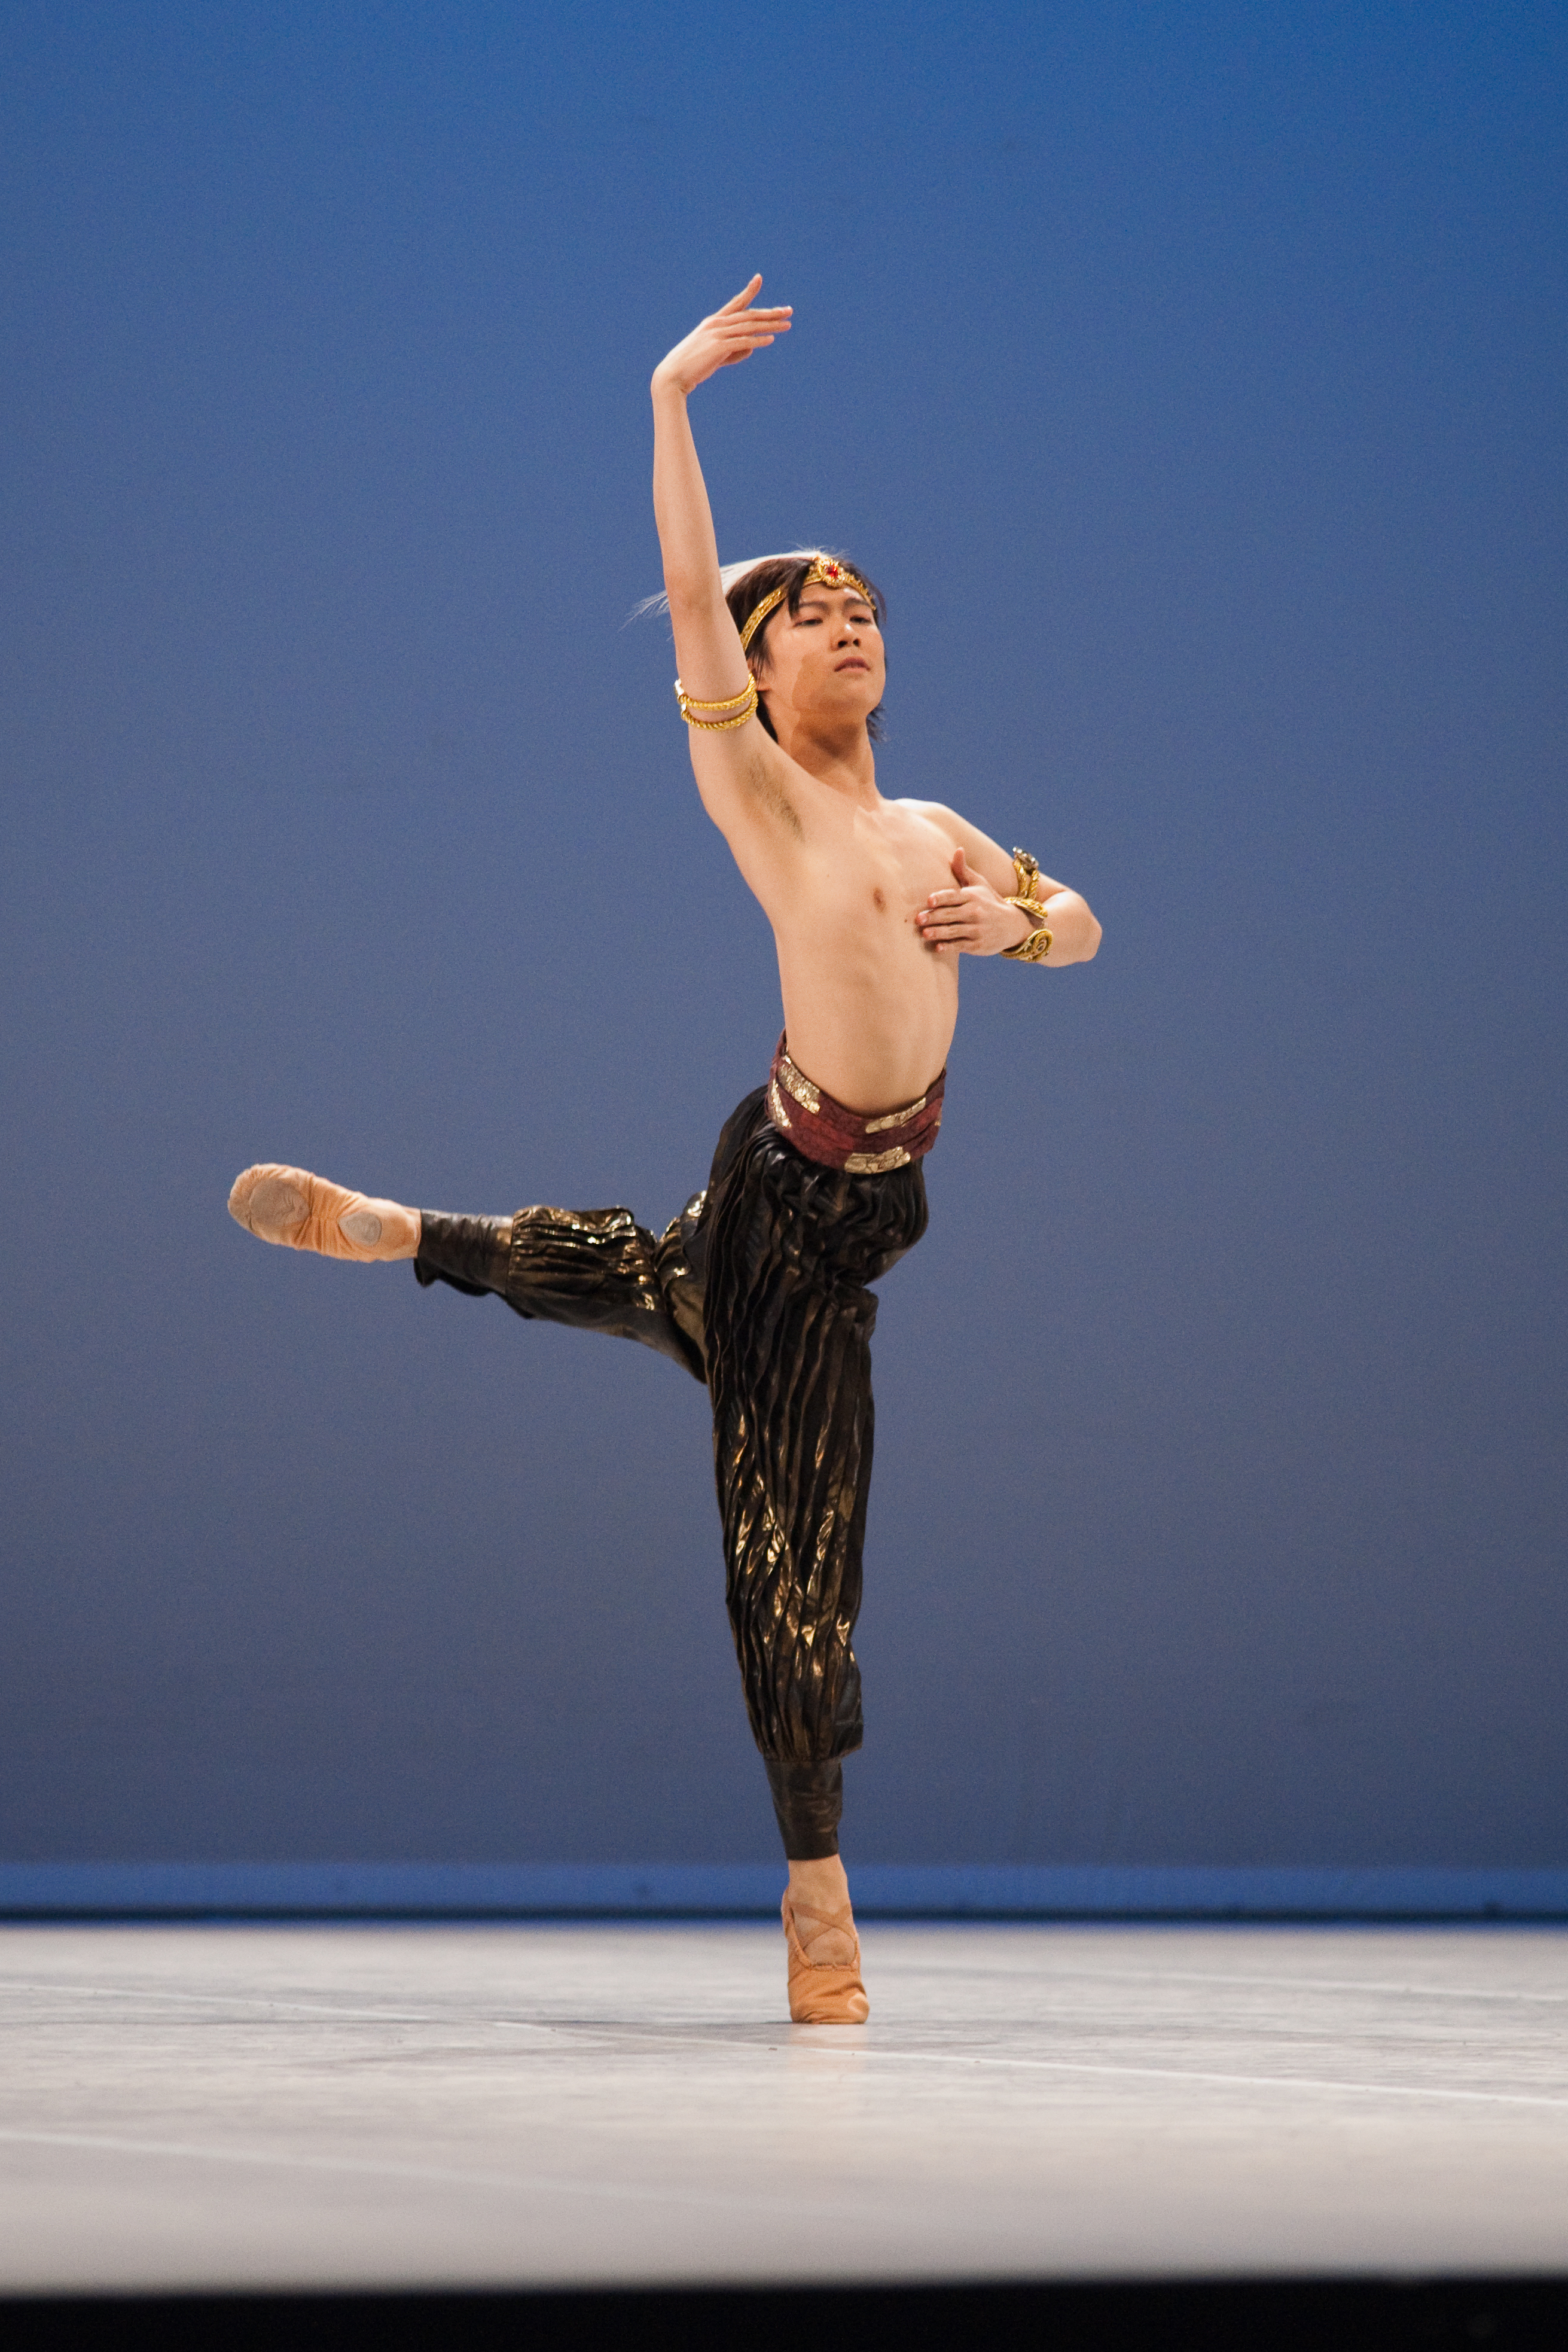
\includegraphics[height=3cm]{../images/Pivot.jpg}
\end{frame} 
 
 
\begin{frame}{}
\begin{block}{Definition (Pivot)}
A pivot is:
\begin{itemize}
\item a function (based on the data and parameters) which always has the same distribution regardless of the value of the parameter, for some statistical model.
\item the random variable from which we construct CIs.
\item often of the form $\frac{Estimate - Parameter}{Standard \; Error} \sim Distribution$
where the $Standard \; Error$ is the standard deviation of the $Estimate$.
\end{itemize}
\end{block}

\vspace{.5cm}
It turns out that the Test Statistics, previously considered in Part 3, can be used as Pivots. Hence, we effectively rearrange the Pivot to get the CI.
\end{frame} 

\subsection[Confidence Intervals]{Overview of Confidence Intervals}
\begin{frame}{Overview of Confidence Intervals}

\begin{block}{Definition (Confidence Interval)}
A Confidence Interval is:
\begin{itemize}
\item a sequence of intervals which contain the unknown parameter $(1-\alpha)$\% of the time, where $\alpha$ is the confidence level, often $\alpha = 0.05$.
\href{https://gauss17gon.shinyapps.io/conf_intervals/}{\beamergotobutton{Sequence of CIs}}
\item of the form $(Point) Estimate \pm Critical Value \times Standard Error$.
\item a set of possible hypotheses $\{ H_{0}: \mu = \mu_{0} \}$, which will be retained if $\mu_{0} \in CI$.
\end{itemize}

\vspace{.5cm}
A Confidence Interval is {\it not} an interval which contains the unknown parameter $(1-\alpha)$\% of the time.
\end{block}
\end{frame}




\subsection[Formulae for Confidence Intervals]{Formulae for Confidence Intervals}
\begin{frame}{Formulae for Confidence Intervals}
\vspace{.5cm}
{\small \begin{tabular}{lll} \hline
Test &  Parameter & Test Statistic and CI \\ \hline
Proportion & $p$ & \framebox{T} $\frac{ \hat{p} - p }{ \sqrt{ \frac{\hat{p}(1-
\hat{p})}{n} }} \sim Z$  \\
& & \framebox{CI} $\hat{p} \pm z^{*} \sqrt{ \frac{\hat{p}(1-
\hat{p})}{n} }$  \mbox{ Approximate} \\ 
& & \framebox{CI} $\hat{p} \pm z^{*} \frac{1}{2 \sqrt{n}}$  \mbox{ Conservative}   \\ \hline \hline
1 sample $Z$ & $\mu$ & \framebox{T} $\frac{ \bar{X} - \mu }{ \frac{\sigma}{\sqrt{n}} } \sim Z$  \\
 &  & \framebox{CI} $\bar{x} \pm z^{*} \frac{\sigma}{\sqrt{n}}$  \\ \hline
1 sample $T$ & $\mu$ & \framebox{T} $\frac{ \bar{X} - \mu }{ \frac{s}{\sqrt{n}} } \sim t_{n-1}$  \\ 
& & \framebox{CI} $\bar{x} \pm t_{n-1}^{*} \frac{s}{\sqrt{n}}$   \\ \hline
2 sample $T$ & $\mu_{1} - \mu_{2}$ & \framebox{T} $\frac{ \bar{X_{1}} - \bar{X_{2}} - (\mu_{1}-\mu_{2}) }{ s_{p} \sqrt{ \frac{1}{n_{1}} + \frac{1}{n_{2}}  } } \sim t_{n_{1} + n_{2}-2}$  \\
& & \framebox{CI}  $\bar{x}_{1} - \bar{x}_{2} \pm t_{n_{1} + n_{2}-2}^{*} s_{p} \sqrt{ \frac{1}{n_{1}} + \frac{1}{n_{2}}  }   $  \\ \hline
\end{tabular}}
\end{frame}



\subsection[Confidence Interval for Mean based on Z test]{Confidence Interval for Mean based on Z Test Statistic}

\begin{frame}[fragile]{Confidence Interval for Mean based on Z Test Statistic}

We will consider this example in detail, and then treat the other CIs by analogy.

\vspace{.5cm}
Assume we have a sample $x_{1}, x_{2}, \ldots, x_{n}$ from a Normal population $X \sim N(\mu, \sigma^2)$, where $\mu$ is unknown and $\sigma^2$ is known.

\vspace{.5cm}
The best estimate of the population mean is the sample mean:
\[ \hat{\mu} = \bar{x} = \frac{\sum_{i=1}^n x_{i}}{n} \]

\vspace{.5cm}
As the sample mean will differ from sample to sample, we want to find a plausible set of values for $\mu$ that incorporates this sample to sample variation.

\end{frame}

\begin{frame}[fragile]{}

Based on the 1 sample $Z$ test statistic, we want to find a 95\% CI. 

\vspace{.5cm}
(1) If $P(-z^{*} \leq Z \leq z^{*}) = 0.95$, we know that $z^{*} = 1.96$. \\


\begin{knitrout}
\definecolor{shadecolor}{rgb}{0.969, 0.969, 0.969}\color{fgcolor}
\includegraphics[width=\maxwidth]{figure/unnamed-chunk-5-1} 
\begin{kframe}\begin{verbatim}
## [1] 1.959964
\end{verbatim}
\end{kframe}
\end{knitrout}
\end{frame}

\begin{frame}[fragile]{}

(2) Now substituting the pivot 
$Z = \frac{ \bar{X} - \mu }{ \frac{\sigma}{\sqrt{n}} }$, gives

\[ P(-z^{*} \leq \frac{ \bar{X} - \mu }{ \frac{\sigma}{\sqrt{n}} } \leq z^{*}) = 0.95 \]

Rearranging gives
\[ P( -\bar{X} -z^{*} \frac{\sigma}{\sqrt{n}}  \leq        -\mu         \leq  -\bar{X} + z^{*} \frac{\sigma}{\sqrt{n}}) = 0.95 \]

which simplifies to

\[ P( \bar{X} -z^{*} \frac{\sigma}{\sqrt{n}}  \leq  \mu  \leq  \bar{X} + z^{*} \frac{\sigma}{\sqrt{n}}) = 0.95 \]
\end{frame}

\begin{frame}[fragile]{}
(3) This is a random interval which covers $\mu$ with probability 0.95. 

\vspace{.5cm}
\begin{center}
\framebox{ $\bar{X}  \pm 1.96 \frac{\sigma}{\sqrt{n}}$ }
\end{center}



\vspace{.5cm}
(4) The observed value of the interval is called the 95\% Confidence Interval (CI) for $\mu$.

\vspace{.5cm}
\begin{center}
\framebox{ $\bar{x}  \pm 1.96 \frac{\sigma}{\sqrt{n}}$ }
\end{center}

(5) More generally, the $(1-\alpha)$\% Confidence Interval (CI) for $\mu$ is:

\vspace{.5cm}
\begin{center}
\framebox{ $\bar{x}  \pm z^{*} \frac{\sigma}{\sqrt{n}}$ }
\end{center}
where $P(-z^{*} \leq Z \leq z^{*}) = 1-\alpha$ or
$P(Z \geq z^{*}) = \frac{\alpha}{2}$.


\end{frame}

\begin{frame}[fragile]{}

\vspace{.5cm}
Note: \\
(1) The CI refers to the proportion of CIs that will cover the true $\mu$ if the above procedure is repeated for many samples of size $n$. We only observe one sample, so we don't know if it is one that contains $\mu$. 

\includegraphics[height=4cm]{../images/CI.jpg} 

\vspace{.5cm}
(2) As we increase $n$, the CI gets narrower, and so $\bar{x}$ is a better estimate for the long term estimate of $\mu$.
\end{frame}

\begin{frame}[fragile]{}

\vspace{.5cm}
(3) As we increase the confidence level, the CI gets wider.
\end{frame}


\begin{frame}[fragile]{}

\begin{alertblock}{Practise finding critical values}
Find $z^{*}$ for 70\%, 80\%, 90\%, 95\% and 99\% CIs.
\end{alertblock}

{\tiny
\begin{knitrout}
\definecolor{shadecolor}{rgb}{0.969, 0.969, 0.969}\color{fgcolor}\begin{kframe}
\begin{alltt}
\hlkwd{qnorm}\hlstd{(}\hlnum{0.85}\hlstd{)}
\end{alltt}
\begin{verbatim}
## [1] 1.036433
\end{verbatim}
\begin{alltt}
\hlkwd{qnorm}\hlstd{(}\hlnum{0.9}\hlstd{)}
\end{alltt}
\begin{verbatim}
## [1] 1.281552
\end{verbatim}
\begin{alltt}
\hlkwd{qnorm}\hlstd{(}\hlnum{0.95}\hlstd{)}
\end{alltt}
\begin{verbatim}
## [1] 1.644854
\end{verbatim}
\begin{alltt}
\hlkwd{qnorm}\hlstd{(}\hlnum{0.975}\hlstd{)}
\end{alltt}
\begin{verbatim}
## [1] 1.959964
\end{verbatim}
\begin{alltt}
\hlkwd{qnorm}\hlstd{(}\hlnum{0.995}\hlstd{)}
\end{alltt}
\begin{verbatim}
## [1] 2.575829
\end{verbatim}
\end{kframe}
\end{knitrout}
}
\end{frame}


\subsection[Worked Examples]{Worked Examples}
\begin{frame}[fragile]{Example1: Birth Weight}

We have $W \sim N(\mu,0.525^2)$ and the data:

\begin{knitrout}
\definecolor{shadecolor}{rgb}{0.969, 0.969, 0.969}\color{fgcolor}\begin{kframe}
\begin{alltt}
\hlstd{x}\hlkwb{=}\hlkwd{c}\hlstd{(}\hlnum{2.853}\hlstd{,}\hlnum{3.127}\hlstd{,}\hlnum{3.159}\hlstd{,}\hlnum{3.800}\hlstd{,}\hlnum{2.656}\hlstd{,}\hlnum{3.245}\hlstd{,}\hlnum{3.510}\hlstd{,}\hlnum{3.082}\hlstd{)}
\hlkwd{mean}\hlstd{(x)}
\end{alltt}
\begin{verbatim}
## [1] 3.179
\end{verbatim}
\end{kframe}
\end{knitrout}

(i) The best estimate for $\mu$ is $\bar{x} = 3.179$ \\

\vspace{.5cm}
(ii) A 95\% CI for $\mu$ is: 
\[ \bar{x}  \pm 1.96 \frac{\sigma}{\sqrt{n}} \] which is $3.179  \pm 1.96 \frac{0.525}{\sqrt{8}}$, giving (2.82,3.54).
\begin{knitrout}
\definecolor{shadecolor}{rgb}{0.969, 0.969, 0.969}\color{fgcolor}\begin{kframe}
\begin{alltt}
\hlkwd{qnorm}\hlstd{(}\hlnum{0.975}\hlstd{)}
\end{alltt}
\begin{verbatim}
## [1] 1.959964
\end{verbatim}
\end{kframe}
\end{knitrout}
\end{frame}

\begin{frame}[fragile]{}

A 99\% CI for $\mu$ is: 
\[ \bar{x}  \pm z^{*} \frac{\sigma}{\sqrt{n}} \]
which is $3.179  \pm 2.576 \frac{0.525}{\sqrt{8}}$, giving (2.70,3.66).

\begin{knitrout}
\definecolor{shadecolor}{rgb}{0.969, 0.969, 0.969}\color{fgcolor}\begin{kframe}
\begin{alltt}
\hlkwd{qnorm}\hlstd{(}\hlnum{0.995}\hlstd{)}
\end{alltt}
\begin{verbatim}
## [1] 2.575829
\end{verbatim}
\end{kframe}
\end{knitrout}

\begin{knitrout}
\definecolor{shadecolor}{rgb}{0.969, 0.969, 0.969}\color{fgcolor}
\includegraphics[width=\maxwidth]{figure/unnamed-chunk-10-1} 

\end{knitrout}
\end{frame}



\begin{frame}[fragile]{Example2: Paint Primer}

We have $X \sim N(\mu,\sigma^2)$ and the data:

\begin{knitrout}
\definecolor{shadecolor}{rgb}{0.969, 0.969, 0.969}\color{fgcolor}\begin{kframe}
\begin{alltt}
\hlstd{x}\hlkwb{=}\hlkwd{c}\hlstd{(}\hlnum{1.30}\hlstd{,}\hlnum{1.10}\hlstd{,}\hlnum{1.20}\hlstd{,}\hlnum{1.25}\hlstd{,}\hlnum{1.05}\hlstd{,}\hlnum{0.95}\hlstd{,}\hlnum{1.10}\hlstd{,}\hlnum{1.16}\hlstd{,}\hlnum{1.37}\hlstd{,}\hlnum{0.98}\hlstd{)}
\hlkwd{mean}\hlstd{(x)}
\end{alltt}
\begin{verbatim}
## [1] 1.146
\end{verbatim}
\begin{alltt}
\hlkwd{sd}\hlstd{(x)}
\end{alltt}
\begin{verbatim}
## [1] 0.1363166
\end{verbatim}
\end{kframe}
\end{knitrout}
\end{frame}

\begin{frame}[fragile]{}
(i) A 95\% CI for $\mu$ is: 
\[ \bar{x}  \pm t^{*} \frac{s}{\sqrt{n}} \]
which is $1.146  \pm 2.262 \frac{0.136}{\sqrt{10}}$, giving (1.05,1.24).

\begin{knitrout}
\definecolor{shadecolor}{rgb}{0.969, 0.969, 0.969}\color{fgcolor}\begin{kframe}
\begin{alltt}
\hlkwd{qt}\hlstd{(}\hlnum{0.975}\hlstd{,}\hlnum{9}\hlstd{)}
\end{alltt}
\begin{verbatim}
## [1] 2.262157
\end{verbatim}
\end{kframe}
\end{knitrout}

(ii) The CI does not contain $H_{0}: \mu=1.25$ hence the data provide evidence against the company's advertising.
\end{frame}

\begin{frame}[fragile]{Example3: Concrete Tensile Strength}

(i)
{\tiny
\begin{knitrout}
\definecolor{shadecolor}{rgb}{0.969, 0.969, 0.969}\color{fgcolor}\begin{kframe}
\begin{alltt}
\hlstd{small}\hlkwb{=}\hlkwd{c}\hlstd{(}\hlnum{4404}\hlstd{,}\hlnum{4326}\hlstd{,}\hlnum{3788}\hlstd{,}\hlnum{3475}\hlstd{,}\hlnum{3418}\hlstd{,}\hlnum{2262}\hlstd{,}\hlnum{7415}\hlstd{,}\hlnum{6993}\hlstd{)}
\hlkwd{mean}\hlstd{(small)}
\end{alltt}
\begin{verbatim}
## [1] 4510.125
\end{verbatim}
\begin{alltt}
\hlkwd{sd}\hlstd{(small)}
\end{alltt}
\begin{verbatim}
## [1] 1792.36
\end{verbatim}
\end{kframe}
\end{knitrout}
}

Assuming that the strengths can be modelled by $N(\mu,1000^2)$, a 95\% CI for the mean tensile strength of small specimens is:
\[ \bar{x}  \pm 1.96 \frac{\sigma}{\sqrt{n}}\]
which is
\[ 4510.125 \pm 1.96*1000/\sqrt{8} \] which gives 
\[ (3817,5203). \]
\end{frame}

\begin{frame}[fragile]{}

(ii)
{\tiny
\begin{knitrout}
\definecolor{shadecolor}{rgb}{0.969, 0.969, 0.969}\color{fgcolor}\begin{kframe}
\begin{alltt}
\hlstd{small}\hlkwb{=}\hlkwd{c}\hlstd{(}\hlnum{4404}\hlstd{,}\hlnum{4326}\hlstd{,}\hlnum{3788}\hlstd{,}\hlnum{3475}\hlstd{,}\hlnum{3418}\hlstd{,}\hlnum{2262}\hlstd{,}\hlnum{7415}\hlstd{,}\hlnum{6993}\hlstd{)}
\hlstd{large}\hlkwb{=}\hlkwd{c}\hlstd{(}\hlnum{4140}\hlstd{,}\hlnum{3984}\hlstd{,}\hlnum{3842}\hlstd{,}\hlnum{3053}\hlstd{,}\hlnum{3145}\hlstd{,}\hlnum{1813}\hlstd{,}\hlnum{6867}\hlstd{,}\hlnum{7091}\hlstd{)}
\hlstd{diff}\hlkwb{=}\hlstd{large}\hlopt{-}\hlstd{small}
\hlkwd{mean}\hlstd{(diff)}
\end{alltt}
\begin{verbatim}
## [1] -268.25
\end{verbatim}
\begin{alltt}
\hlkwd{sd}\hlstd{(diff)}
\end{alltt}
\begin{verbatim}
## [1] 232.3893
\end{verbatim}
\end{kframe}
\end{knitrout}
}

Assuming that the differences can be modelled by $N(\mu,\sigma^2)$, a 90\% CI for the mean difference in tensile strengths is:
\[ \bar{x}  \pm t^{*}_{7} \frac{s}{\sqrt{n}} \]
which is
$-268.25 \pm 1.895*232.39/\sqrt{8}$ which gives (113,424).

\begin{knitrout}
\definecolor{shadecolor}{rgb}{0.969, 0.969, 0.969}\color{fgcolor}\begin{kframe}
\begin{alltt}
\hlkwd{qt}\hlstd{(}\hlnum{0.95}\hlstd{,}\hlnum{7}\hlstd{)}
\end{alltt}
\begin{verbatim}
## [1] 1.894579
\end{verbatim}
\end{kframe}
\end{knitrout}
\end{frame}


\begin{frame}[fragile]{Example4: Clinton vs Trump Polls}

Given a random survey of 2000 voters found that 1165 were going to vote for Clinton:

\vspace{.5cm}
(i) A 95\% approximate CI for the proportion of voters $p$ that will vote for Hillary is:
\[ \hat{p} \pm Z^{*} \sqrt{ \frac{\hat{p}(1-
\hat{p})}{n}} \]

Given $\hat{p} = 1165/2000 = 0.5825$, we get \\
\[ 0.5825 \pm 1.96 \sqrt{ \frac{0.5825*(1-0.5825)}{2000}} \]
which gives
\[ (0.56,0.60) \].
\end{frame}

\begin{frame}[fragile]{}

A 95\% conservative CI for the proportion of voters $p$ that will vote for Hillary is:
\[ \hat{p} \pm Z^{*} \frac{1}{2 \sqrt{n}} \]
which is
\[ 0.5825 \pm 1.96 \frac{1}{2 \sqrt{2000}} \]
which gives
\[ (0.56,0.60). \]

\vspace{.5cm}
(ii) The `margin of error' is $1.96 \frac{1}{2 \sqrt{2000}}$
which is 0.02191347 or approximately 2\%.

\end{frame}

\begin{frame}[fragile]{}

\vspace{.5cm}
(iii) To give a 95\% CI for $p$ with width $\pm 0.03$ (ie margin of error 3\%):

We solve \[ 1.96 \frac{1}{2 \sqrt{n}} = 0.03 \]
which gives
\[ n = (\frac{1.96}{2 (0.03)} )^2 \]
resulting in $n=1067$, or approximately 1000.

\vspace{.5cm}
Note that  $1.96 \frac{1}{2 \sqrt{n}} \approx \frac{1}{\sqrt{n}}$, so the margin of error is approximately $\frac{1}{\sqrt{n}}$, which clearly decreases for larger $n$.
\end{frame}




\subsection[Justifying the Conservative CI for Proportion]{Justifying the Conservative CI for Proportion}
\begin{frame}[fragile]{Justifying the Conservative CI for Proportion}

The Standard Error in the Approximate CI is $\sqrt{ \frac{\hat{p}(1- \hat{p})}{n} }$. \\

As $0 \leq \hat{p} \leq 1$, then
 $0 \leq \hat{p}(1- \hat{p}) \leq \frac{1}{4}$, as the maximum of the function occurs when $\hat{p} = \frac{1}{2}$.
 
\begin{knitrout}
\definecolor{shadecolor}{rgb}{0.969, 0.969, 0.969}\color{fgcolor}
\includegraphics[width=\maxwidth]{figure/unnamed-chunk-16-1} 

\end{knitrout}
 
Hence,the maximum that the SE can be is 
$\sqrt{ \frac{\frac{1}{4}}{n} } = \frac{1}{2 \sqrt{n}}$
which is what we use in the conservative CI. That is, we choose the largest possible CI.
\end{frame}
\end{document}
